\documentclass[11pt]{article}

% ------------------------------------------------------------------
% A pluripotency-domain benchmark of temporal trajectory inference.
% Compile:  pdflatex benchmark_manuscript.tex (x2)
% Figures expected in ./figures_v2/ ; bibliography inline (no .bib).
% All numbers read from benchmark/reports/, benchmark/results/,
% and results/annotation_branch/. Nothing is fabricated.
% ------------------------------------------------------------------

\usepackage[utf8]{inputenc}
\usepackage[T1]{fontenc}
\usepackage{lmodern}
\usepackage[margin=1in]{geometry}
\usepackage{graphicx}
\usepackage{booktabs}
\usepackage{multirow}
\usepackage{amsmath}
\usepackage{amssymb}
\usepackage{array}
\usepackage[font=small,labelfont=bf]{caption}
\usepackage{authblk}
\usepackage{microtype}
\usepackage[round,authoryear]{natbib}
\usepackage{xcolor}
\usepackage[colorlinks=true,allcolors=blue!55!black]{hyperref}

\newcommand{\code}[1]{\texttt{\small #1}}
\captionsetup{labelsep=period}
\setlength{\parskip}{0.4em}
\setlength{\parindent}{0pt}

\title{\bfseries Does it transfer? A pluripotency-domain benchmark of temporal
trajectory-inference methods across iPSC reprogramming systems, with
scANVI-validated cell-state references}

\author[1]{Kuma\thanks{Corresponding author. Co-authors and affiliations to be
added.}}
\affil[1]{\small Graduate School of Frontier Sciences, The University of Tokyo}
\date{Working draft, June 2026}

\begin{document}
\maketitle

\begin{abstract}
\noindent
scTimeBench \citep{osakwe2026} established that temporal single-cell
trajectory-inference methods should be judged on three tasks --- forecast accuracy,
embedding coherence, and lineage fidelity --- and showed, across heterogeneous
developmental datasets, that strong forecasters need not preserve biology and that
lineage fidelity is the hardest task. We narrow the benchmark to a single biological
domain --- \textbf{induced pluripotency} --- and make the
reprogramming/differentiation modality the experimental axis, assembling time-labeled
iPSC scRNA-seq datasets that reach or leave the pluripotent state by distinct routes,
to ask whether a method's ranking \emph{transfers} across them. Because most iPSC
datasets lack per-cell author labels, we also contribute a
reference-construction-and-validation pipeline: silver cell-state references are built
by scANVI/scArches label transfer and screened by a geometric out-of-distribution
(OOD) gate, computed inside the main pipeline, that quantifies when a transferred
reference can be trusted. Three findings stand out. \textbf{(1)~Transferred references
fail detectably across modality.} A cross-modality transfer collapses --- the geometric
OOD gate flags $73$--$76\%$ of query cells while scANVI's classifier confidence flags
$\leq0.3\%$ --- so references are accepted only for within-modality transfers (agreement
$0.76$--$0.86$; labeled self-transfer $0.94$), the regime the benchmark itself
recommends. \textbf{(2)~Lineage rankings do not transfer across systems.} Recovery
against the frozen coarse reference graphs reorders the methods from one system to the
next; across the four marker-silver systems lineage rankings are near-discordant
(Kendall's $W=0.19$), with the top and bottom projection-capable methods swapping places
between a mouse and a human-blood system, whereas forecast rankings stay comparatively
stable ($W=0.75$). \textbf{(3)~Single-seed leaderboards are unstable.} Across five seeds
the lineage leader on the primary datasets changes, and single-seed values frequently
fall outside the 5-seed 95\% confidence interval; a diffusion-pseudotime axis can
sharpen recovery (most strikingly PRESCIENT on GSE230659) but the gain is method- and
system-dependent. The practical message is that in this domain a method should be chosen
per task and validated on a system close to the target biology --- a lineage result in
particular should not be read off a single averaged leaderboard. All datasets are public;
reported numbers are read from synced result files, with multi-seed intervals provided as
derived artifacts (Section~\ref{sec:repro}).
\end{abstract}

% ------------------------------------------------------------------
\section{Introduction}
% ------------------------------------------------------------------
Temporal single-cell methods project cells from one observed time point to the next,
and benchmarking them is hard because each cell is measured once, so the ``truth'' for
a projected cell must be assembled from held-out time points and reference
annotations. scTimeBench \citep{osakwe2026} formalized this with three tasks ---
forecast accuracy, embedding coherence, and lineage fidelity --- across eight
developmental datasets spanning four species, concluding that strong forecasters often
fail to preserve latent-space and lineage structure, and that lineage recovery is the
central weakness, with methods frequently no better than a Spearman-correlation
baseline.

scTimeBench answers ``which method is best on average across developmental systems?''.
We ask two questions it does not. \textbf{(1) Within one domain, does method
performance transfer across biological routes?} Induced pluripotency is reached or
left by mechanistically distinct paths --- chemical reprogramming, OSKM
transcription-factor reprogramming, directed differentiation, and organoid development
--- that share the pluripotent state. If a method's ranking is stable across these
routes, a practitioner can choose once; if it inverts, method choice must be
conditioned on the system. \textbf{(2) How do we benchmark on the many iPSC datasets
that lack author labels?} Embedding coherence and lineage fidelity both need a
cell-state reference, yet two of our primary datasets ship none. We address this with a
scANVI/scArches label-transfer pipeline gated by a geometric out-of-distribution
score, which lets the benchmark scale to unlabeled data while measuring when a
transferred reference can be trusted. These are the two innovations that distinguish
this work from scTimeBench.

% ------------------------------------------------------------------
\section{Methods}
% ------------------------------------------------------------------

\subsection{Datasets: the iPSC suite and its run status}
The benchmark spans six time-labeled iPSC scRNA-seq datasets across reprogramming and
differentiation modalities, plus a human cerebral-organoid time course held out as a
planned extension (Table~\ref{tab:data}). Run status is heterogeneous and stated
per-dataset rather than aggregated: four datasets carry completed formal runs across
all three tasks (the two human chemical primaries and the mouse and human-blood
cross-system datasets), GSE242424 (OSKM) carries all three tasks under a separate
author-cluster reference protocol (Section~\ref{sec:refval}), GSE175634 carries
forecast and embedding only, and the organoid course is integration-ready but not yet
run. All are public; provenance and per-task run status are in
\code{datasets/dataset\_inventory.\{md,csv\}}.

\begin{table}[ht]
\centering
\caption{The pluripotency-domain dataset suite (six iPSC datasets plus an organoid
extension). ``Run status'' is the honest state of the synced results.}
\label{tab:data}
\small
\begin{tabular}{l l l c l}
\toprule
Accession & System & Modality & Cells & Run status \\
\midrule
GSE178325 & human hADSC$\to$hCiPS & chemical reprog. & 80{,}475 & results (all 3 tasks) \\
GSE230659 & human hADSC$\to$hCiPS & chemical reprog. & 75{,}194 & results (all 3 tasks) \\
GSE242424 & human fibroblast$\to$iPSC & OSKM reprog. & 59{,}187 & results (all 3 tasks) \\
GSE175634 & human iPSC$\to$cardiomyocyte & differentiation & 224{,}202 & forecast + embedding \\
GSE298212 & human blood$\to$hCiPS & chemical reprog. & 38{,}517 & results (all 3 tasks) \\
GSE218855 & mouse MEF$\to$iPSC & chemical reprog. & 54{,}380 & results (all 3 tasks) \\
\midrule
E-MTAB-7552 & human cerebral organoid & organoid (extension) & $\sim$43{,}498 & integration-ready \\
\bottomrule
\end{tabular}
\end{table}

\subsection{Tasks and metrics (inherited from scTimeBench)}
Forecast Accuracy uses the four \code{geomloss} metrics (Wasserstein, Gaussian MMD,
Energy-MMD, Hausdorff), recomputed centrally
(\code{metric\_backend=scTimeBench\_exact}) from each method's standardized
\code{projected\_expression.npy}. Embedding Coherence reports the ARI of Leiden
clusters on the projected embedding against reference labels plus the average
normalized classifier entropy. Lineage Fidelity binarizes the predicted
state-transition matrix at the precision/recall-maximizing threshold and scores
single-step and multi-step (Floyd--Warshall reachability) AUROC, AUPRC, and Jaccard
against the reference graph.

\subsection{Methods and capability gating}
Following scTimeBench's rule that methods are scored only on supported dimensions
(Table~\ref{tab:methods}), the two optimal-transport methods are lineage-only; the
projection-capable methods are scored on all three tasks. CellRank2 \citep{weiler2024}
runs as fate/lineage post-processing on the WOT \citep{schiebinger2019}
\code{RealTimeKernel} and is reported as such. Five projection-capable or lineage-only
methods carry completed runs and constitute the evaluated roster
(Table~\ref{tab:methods}). Three further generative models from the scTimeBench roster
--- scIMF \citep{jiang2026scimf} (a Transformer + interacting mean-field neural SDE),
PI-SDE \citep{jiangwan2024pisde} (a physics-informed neural SDE), and
Squidiff \citep{he2026squidiff} (a conditional diffusion model) --- are scoped as
\textbf{planned extensions}: their adapter interfaces, runtime configs, and Shirokane
job are in the repository, but the model code is not yet vendored (the adapters raise
an explicit \code{VendoringRequired} contract), so these methods are \emph{not}
evaluated here and are excluded from every results table and figure. They are listed
separately below to document the intended capability gating, not as integrated results.

\begin{table}[ht]
\centering
\caption{Method roster and scTimeBench capability gating. The upper block is the
evaluated roster (completed runs); the lower block lists planned extensions whose model
code is not yet vendored and which appear in no results table or figure.}
\label{tab:methods}
\small
\begin{tabular}{l l c l}
\toprule
Method & Algorithm & Projection-capable & Dimensions scored \\
\midrule
\multicolumn{4}{l}{\emph{Evaluated roster (completed runs)}}\\
WOT        & Optimal transport                        & No  & Lineage only \\
CellRank2  & Fate mapping on WOT \code{RealTimeKernel} & No  & Lineage only \\
scNODE     & VAE + neural ODE                         & Yes & All three \\
PRESCIENT  & PCA + neural SDE                         & Yes & All three \\
MIOFlow    & Geodesic VAE + neural ODE                & Yes & All three \\
\midrule
\multicolumn{4}{l}{\emph{Planned extensions (adapter contract only --- not evaluated here)}}\\
scIMF      & Transformer + interacting mean-field SDE & Yes & (planned: all three) \\
PI-SDE     & Physics-informed neural SDE              & Yes & (planned: all three) \\
Squidiff   & Conditional diffusion (PCA space)        & Yes & (planned: all three) \\
\bottomrule
\end{tabular}
\end{table}

\subsection{Scenarios}
For each dataset, Scenario~A is observed-time interpolation, Scenario~B is
extrapolation to later unseen time points, and Scenario~C is the joint setting;
metrics are computed on held-out time points. Scenarios~D/E/F repeat the same
interpolation/extrapolation/joint splits on a 15-bin diffusion-pseudotime axis
(Scanpy DPT, rooted at the earliest observed time point), testing whether
ordering cells by an inferred internal clock improves recovery.

\subsection{Reference construction and validation (the scANVI integration)}
\label{sec:refval}
Because the chemical-reprogramming primaries ship no per-cell author labels, silver
references are built by scANVI/scArches \citep{xu2021,lotfollahi2022} label transfer
from an annotated atlas and screened by three gates: a \textbf{self-recovery gate}
(scANVI must re-predict the reference's own labels at $\geq0.90$; met on GSE242424 at
$0.990$), a \textbf{geometric OOD gate} (each query cell's mean distance to its $k$
nearest reference cells in the shared latent, referenced against the reference's own
kNN-distance distribution; a cell is flagged when it falls beyond the reference's
$q$-quantile, with defaults $k=15$, $q=0.95$), and a \textbf{within-modality rule}.
The geometric gate is computed inside the main pipeline (\code{src/pipeline.py} calls
\code{src/annotation/ood.py}) and reported alongside the classifier-confidence flag, so
each run emits both the global OOD fraction and a per-state breakdown; the same routine
runs on the server scANVI latent via \code{scripts/score\_ood.py}, which is now a thin
wrapper over the shared gate. The threshold parameters $(k,q)$ are configurable; a
sensitivity sweep (\code{scripts/ood\_sensitivity\_sweep.py}, on the local PCA-latent
proxy) shows the cross-modality reject decision is not an artifact of these choices ---
the chemical query is flagged $6.5$--$9.7\times$ more often than the reference's own
self-flag baseline across every $k\in\{5,15,30,50\}$ and $q\in\{0.90,0.95\}$,
collapsing toward parity only in the extreme $q=0.99$ tail where the proxy cannot
resolve the boundary. Accepted transfers seed the frozen \code{official\_silver} provider;
rejected (cross-modality) cases fall back to marker-defined references. The unit-tested
utilities are in \code{src/annotation/}.

% ------------------------------------------------------------------
\section{Results}
% ------------------------------------------------------------------

\subsection{No method dominates all three tasks}
On the two chemical-reprogramming datasets, the combined embedding-plus-lineage
ranking over the projection-capable methods is narrow --- MIOFlow first (combined rank
score $1.79$), PRESCIENT second ($1.85$), scNODE third ($2.18$) --- but the per-task
picture is split (Table~\ref{tab:primary}): PRESCIENT has the most coherent embeddings
(mean ARI $0.135$), MIOFlow recovers lineage best (mean single-step AUROC $0.662$),
and forecast accuracy has no single winner (scNODE wins Scenario~A on both datasets;
PRESCIENT wins the harder B/C on GSE230659). The best forecaster is not the best
lineage recoverer --- the central scTimeBench observation, reproduced on reprogramming
data.

\begin{table}[ht]
\centering
\caption{Primary chemical-reprogramming benchmark (GSE178325 + GSE230659, Scenarios
A/B/C), projection-capable methods. Means over datasets and scenarios; higher ARI and
AUROC are better.}
\label{tab:primary}
\small
\begin{tabular}{l c c c c}
\toprule
Method & Combined rank score & Mean embedding ARI & Mean single-step AUROC & Best at \\
\midrule
MIOFlow   & \textbf{1.79} & 0.072 & \textbf{0.662} & Lineage fidelity \\
PRESCIENT & 1.85 & \textbf{0.135} & 0.630 & Embedding coherence \\
scNODE    & 2.18 & 0.054 & 0.597 & Forecast (Scenario A) \\
\bottomrule
\end{tabular}
\end{table}

\begin{figure}[ht]
\centering
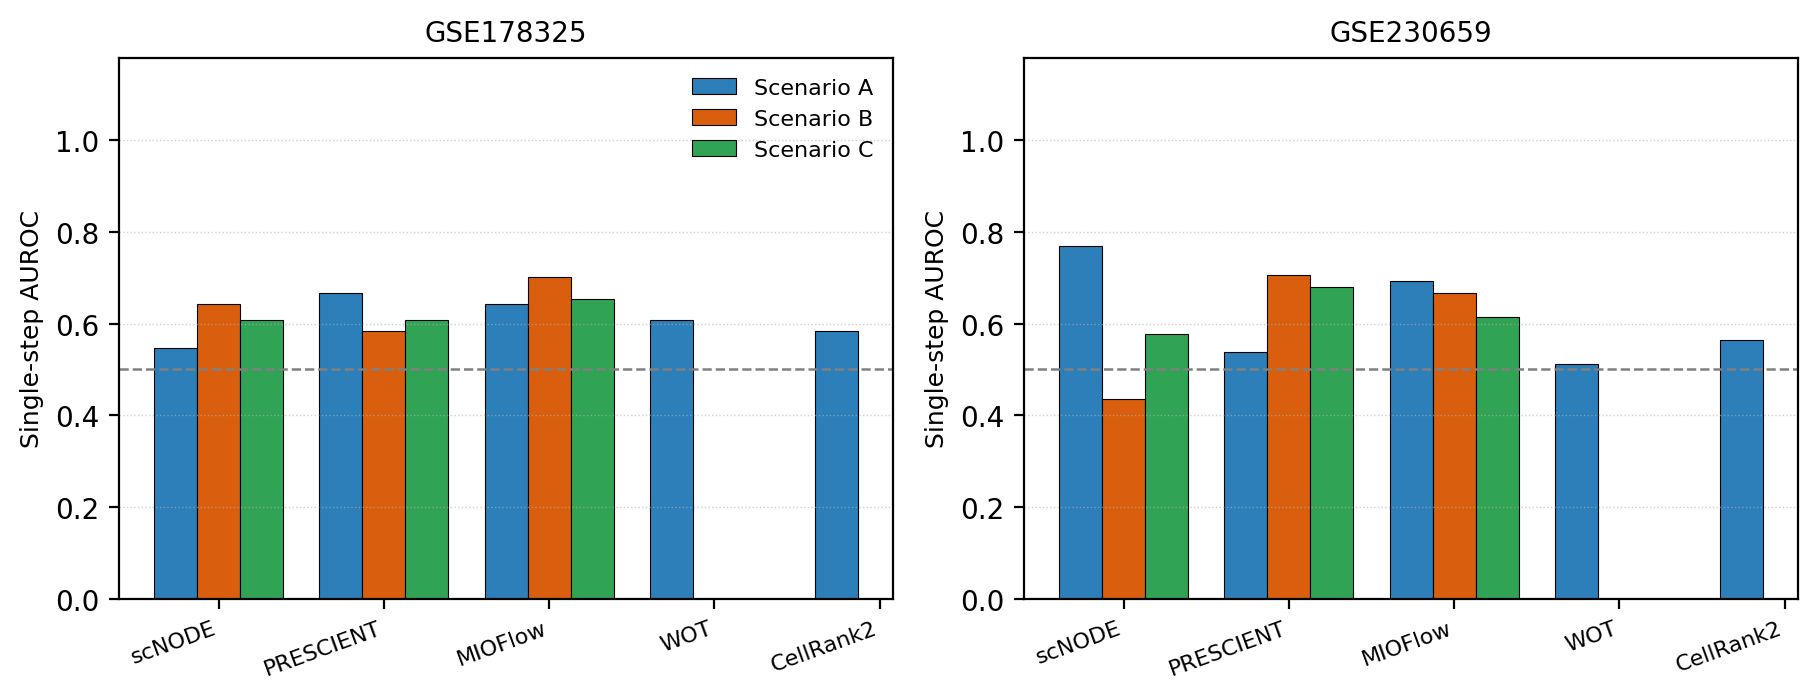
\includegraphics[width=0.95\linewidth]{figures_v2/fig1_lineage_auroc.png}
\caption{Lineage Fidelity (graph-sim single-step AUROC) by method and scenario for the
two chemical datasets. WOT/CellRank2 are lineage-only (run for Scenario~A). Absolute
AUROC stays in a modest $0.44$--$0.77$ band; the dashed line is chance.}
\label{fig:lineage}
\end{figure}

\subsection{Forecasting difficulty: extrapolation degrades every method}
Scenario~B is the universal hard case (Fig.~\ref{fig:forecast}): on GSE230659 the
forecast Wasserstein distance rises from $\approx81$ (scNODE, A) to $148$--$404$ (B),
and the lowest lineage AUROC in the primary benchmark --- scNODE on GSE230659~B at
$0.436$ --- falls below chance. Early-only training leaves the late reprogramming
milestones unobserved, and extrapolation is exposed to library-specific shifts.

\begin{figure}[ht]
\centering
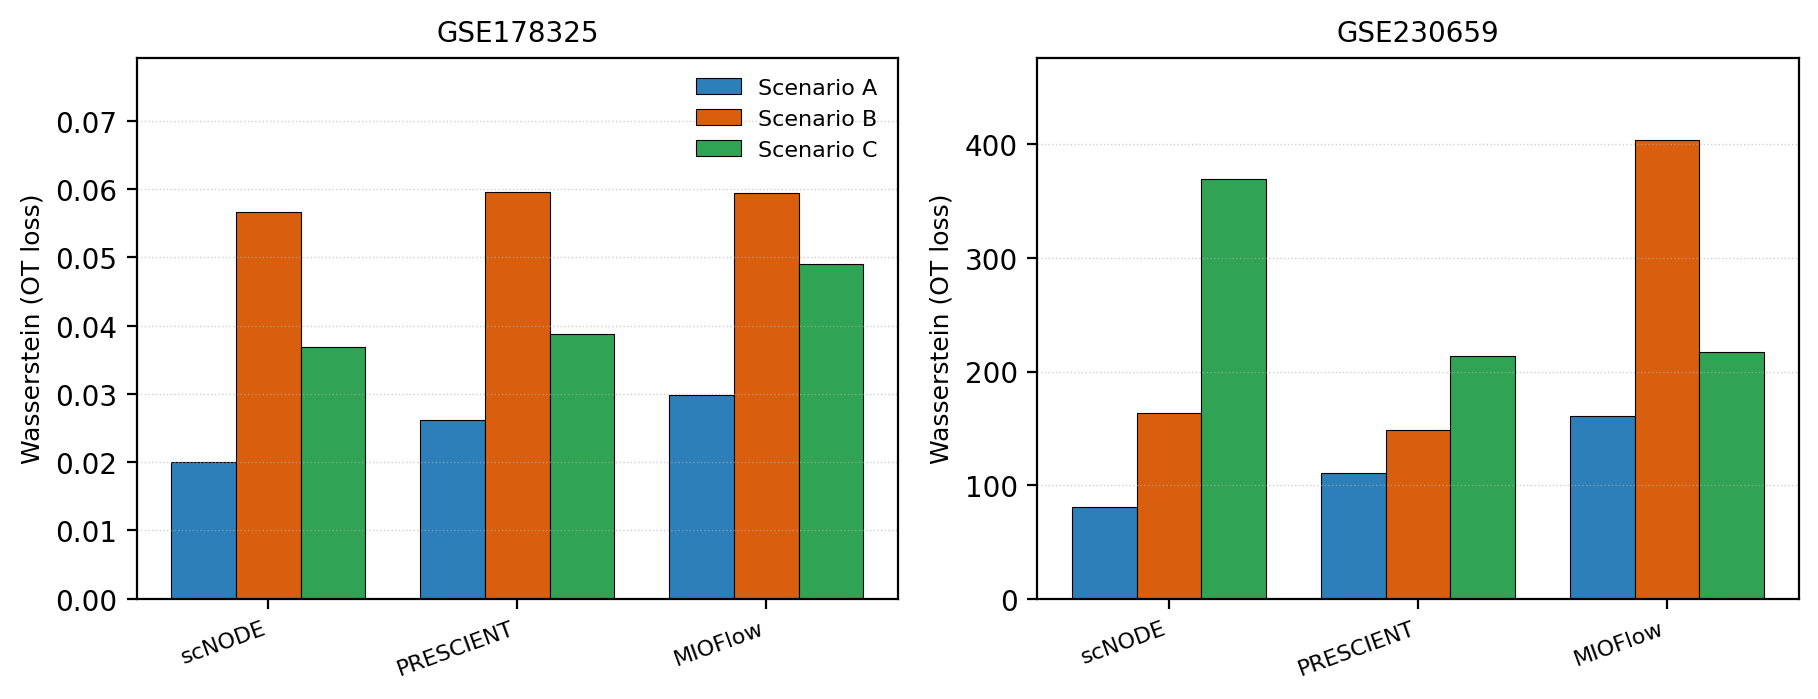
\includegraphics[width=0.95\linewidth]{figures_v2/fig2_forecast_wd.png}
\caption{Forecast Accuracy (exact OT-loss Wasserstein, lower is better) by method and
scenario; the extrapolation setting inflates the loss for all methods. Note the
different vertical scales.}
\label{fig:forecast}
\end{figure}

\subsection{Cross-modality generalization: rankings do not transfer}
The headline result of the pluripotency-domain design is that the \emph{same} methods
behave very differently across reprogramming routes (Fig.~\ref{fig:crosssys}). Lineage
single-step AUROC on the OSKM system (GSE242424) reaches $0.85$ (Scenario~A) with
method means of $0.71$--$0.78$, versus $0.59$--$0.66$ on chemical GSE230659 --- and the
method ordering is not preserved. Lineage performance is therefore as much a property
of the biological system and its reference-graph structure as of the method: a single
averaged leaderboard would hide this, and a method validated on one reprogramming route
cannot be assumed to rank the same on another. Figure~\ref{fig:crosssys} shows the same
instability across all five systems; the next two subsections extend it beyond
reprogramming route to a different species and starting cell type, and put a
concordance statistic on it.

\begin{figure}[ht]
\centering
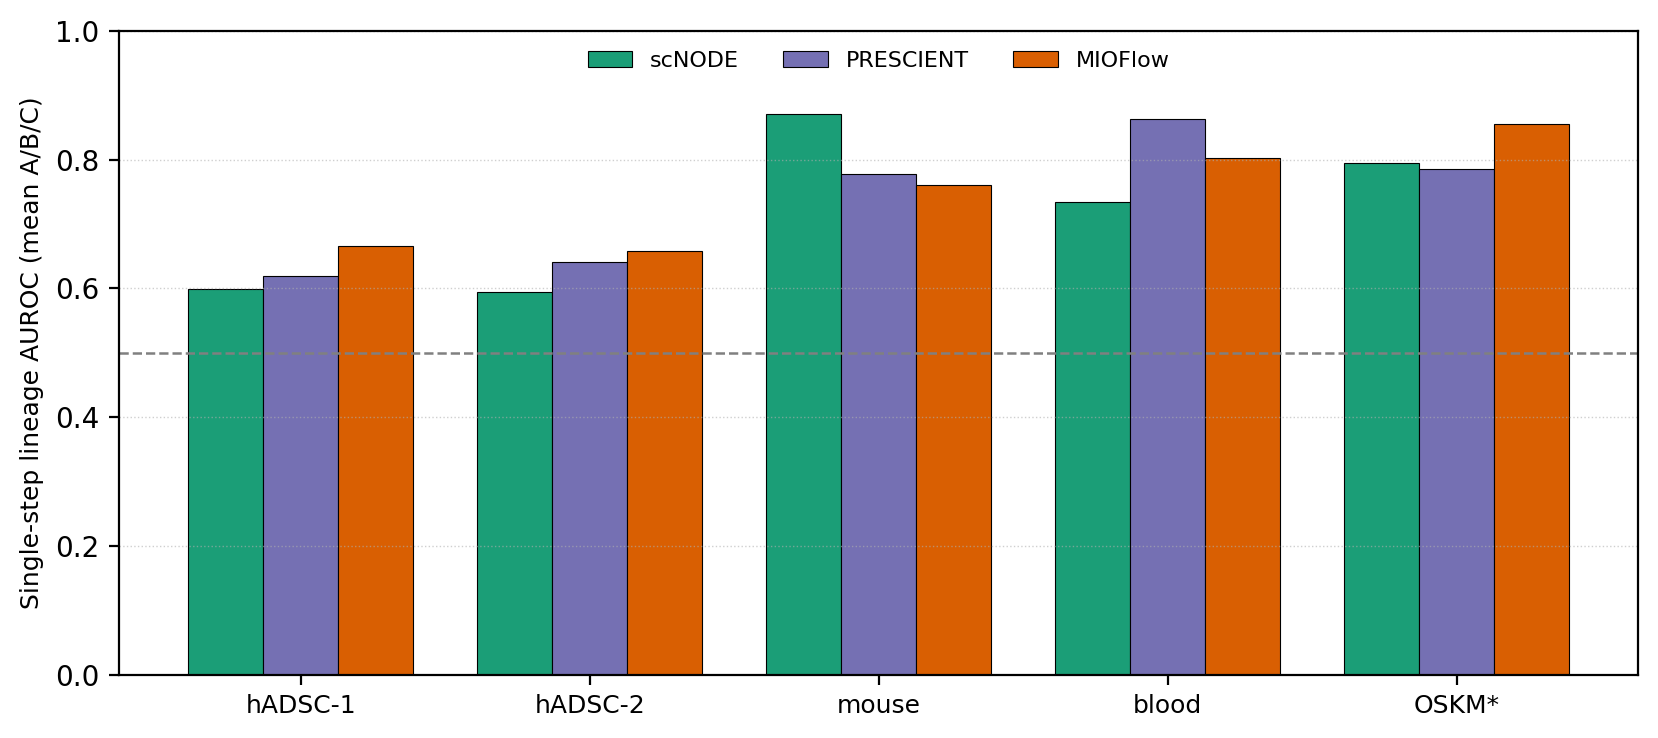
\includegraphics[width=0.80\linewidth]{figures_v2/fig4_cross_system.png}
\caption{Cross-system generalization. Lineage single-step AUROC (mean over A/B/C) for
the three projection-capable methods across the four marker-silver systems (hADSC-1
= GSE178325, hADSC-2 = GSE230659, mouse = GSE218855, blood = GSE298212) and the OSKM
system (GSE242424; ${}^{*}$evaluated under the author-cluster reference protocol, so
its AUROC is not strictly comparable to the marker-silver bars). The leading method
changes from MIOFlow (hADSC) to scNODE (mouse) to PRESCIENT (blood); absolute AUROC is
also markedly higher away from the two hADSC systems.}
\label{fig:crosssys}
\end{figure}

\subsection{Cross-system replication: the ranking flip generalizes to mouse and blood}
Extending the suite beyond a single species and starting cell type sharpens the same
conclusion (Table~\ref{tab:crosssystem}). On the mouse MEF$\to$iPSC system (GSE218855),
scNODE is the strongest projection-capable lineage method (mean single-step AUROC
$0.87$ over A/B/C) and PRESCIENT the weakest ($0.78$); on the human blood$\to$hCiPS
system (GSE298212) the order \emph{inverts} --- PRESCIENT leads ($0.86$) and scNODE
trails ($0.74$). The embedding-coherence ordering flips too (PRESCIENT best on mouse at
ARI~$0.23$, MIOFlow best on blood at $0.17$), while forecast error stays tightly bunched
on both (Wasserstein $0.075$--$0.076$ on mouse, $0.044$--$0.054$ on blood). The
lineage-only optimal-transport baselines remain competitive at the trajectory-root
scenario (CellRank2 single-step AUROC $0.92$ on mouse, $0.82$ on blood). That the top
and bottom generative methods swap places between a mouse and a human system --- neither
of which shares the hADSC starting state used to develop the methods --- is direct
evidence that a leaderboard from one system does not transfer, now replicated across
species and across starting cell type rather than reprogramming route alone.

\begin{table}[ht]
\centering
\caption{Cross-system replication on the two added datasets. Mean over Scenarios A/B/C
for the three projection-capable methods (single-step lineage AUROC, exact OT-loss
forecast Wasserstein [lower better], embedding-coherence ARI). The lineage ordering
inverts between the mouse and human-blood systems.}
\label{tab:crosssystem}
\small
\begin{tabular}{l l c c c}
\toprule
Dataset & Method & Lineage AUROC & Forecast WD & Embed.\ ARI \\
\midrule
\multirow{3}{*}{GSE218855 (mouse)}
 & scNODE    & \textbf{0.87} & 0.075 & 0.14 \\
 & PRESCIENT & 0.78 & 0.075 & \textbf{0.23} \\
 & MIOFlow   & 0.76 & 0.076 & 0.19 \\
\midrule
\multirow{3}{*}{GSE298212 (blood)}
 & scNODE    & 0.74 & 0.045 & 0.06 \\
 & PRESCIENT & \textbf{0.86} & \textbf{0.044} & 0.09 \\
 & MIOFlow   & 0.80 & 0.054 & \textbf{0.17} \\
\bottomrule
\end{tabular}
\end{table}

\subsection{Ranking (in)stability is task-dependent}
To put a statistic on the transfer question we rank the three projection-capable
methods within each of the four marker-silver datasets (mean over Scenarios A/B/C)
and compute Kendall's coefficient of concordance $W$ across datasets, separately for
each task (Fig.~\ref{fig:concordance}). The three tasks behave very differently.
Lineage fidelity is the \emph{least} stable: $W=0.19$, near the no-agreement floor ---
the two human hADSC$\to$hCiPS systems rank the methods identically (pairwise Spearman
$\rho=+1.0$), but the mouse system inverts that order completely ($\rho=-1.0$ against
both), and the human-blood system sits in between. Forecast accuracy is the
\emph{most} stable ($W=0.75$: scNODE/PRESCIENT tend to lead the OT-loss everywhere),
with embedding coherence intermediate ($W=0.56$). A single averaged lineage
leaderboard is therefore actively misleading, whereas a forecast leaderboard
generalizes better --- a distinction a one-number summary would erase. The same
scope-sensitivity appears in the combined embedding-plus-lineage rank: MIOFlow leads
on the observed-time primary benchmark (Table~\ref{tab:primary}), but PRESCIENT takes
first once the pseudotime scenarios or the mouse/blood systems enter the pool. Which
method ``wins'' is a function of the evaluation scope, not a fixed property.

\begin{figure}[ht]
\centering
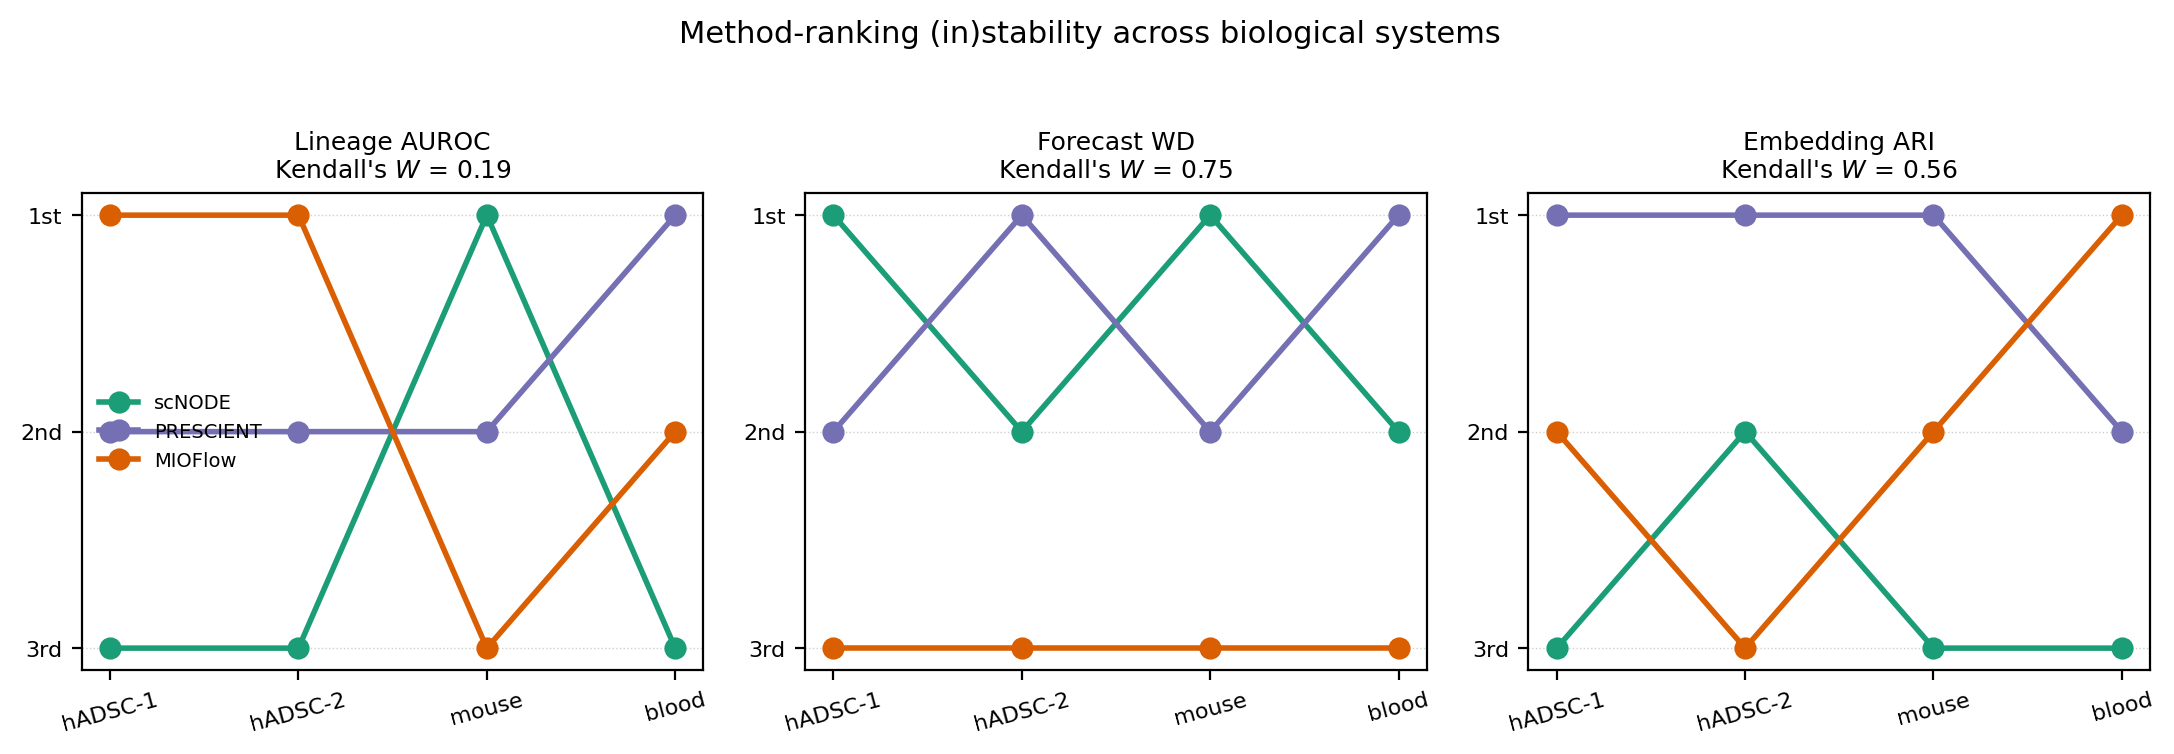
\includegraphics[width=0.95\linewidth]{figures_v2/fig7_rank_concordance.png}
\caption{Method-ranking (in)stability across the four marker-silver systems
(hADSC-1 = GSE178325, hADSC-2 = GSE230659, mouse = GSE218855, blood = GSE298212).
Each line tracks one method's within-dataset rank (mean over A/B/C); Kendall's $W$ is
annotated per task. Lineage rankings cross repeatedly ($W=0.19$); forecast rankings
are nearly flat ($W=0.75$).}
\label{fig:concordance}
\end{figure}

\subsection{Robustness: seed sensitivity and a correlation floor}
Two sanity checks qualify the point estimates above. First, repeating the primary
runs across five random seeds (same hyperparameters; Fig.~\ref{fig:robust}) shows the
single-seed leaderboard is not robust. Averaged over seeds, the best lineage recoverer
on the two chemical primaries is \emph{PRESCIENT} (mean single-step AUROC $0.78$), not
MIOFlow ($0.75$) or scNODE ($0.71$) --- the reverse of the single-seed ordering in
Table~\ref{tab:primary}, and the single-seed values (open circles) frequently fall
outside the 5-seed 95\% confidence interval. The seed sensitivity is itself
method-specific: PRESCIENT's lineage output is essentially seed-invariant (per-scenario
SD $\leq0.008$), whereas MIOFlow's forecast Wasserstein on GSE230659 swings wildly
(Scenario~B mean $529$, 95\% CI $\pm203$). That even the random seed can flip the
lineage leader is the strongest form of the instability this benchmark documents, and
it means single-run leaderboards in this domain should be read as draws, not rankings.

Second, the scTimeBench Spearman correlation baseline (adjacent-timepoint, maximum-vote)
sets a floor every method should clear. It is low on the two human hADSC systems
(single-step AUROC $0.45$ and $0.50$), which all methods beat comfortably, but high on
the cross-system datasets ($0.72$ mouse, $0.79$ blood) --- where the methods only
marginally exceed it (mouse means $0.76$--$0.87$; blood $0.74$--$0.86$). Much of the
apparently strong off-domain lineage recovery is thus attributable to simple
adjacent-timepoint expression similarity rather than learned dynamics, reinforcing
scTimeBench's caution that lineage fidelity is the field's weakest task.

\begin{figure}[ht]
\centering
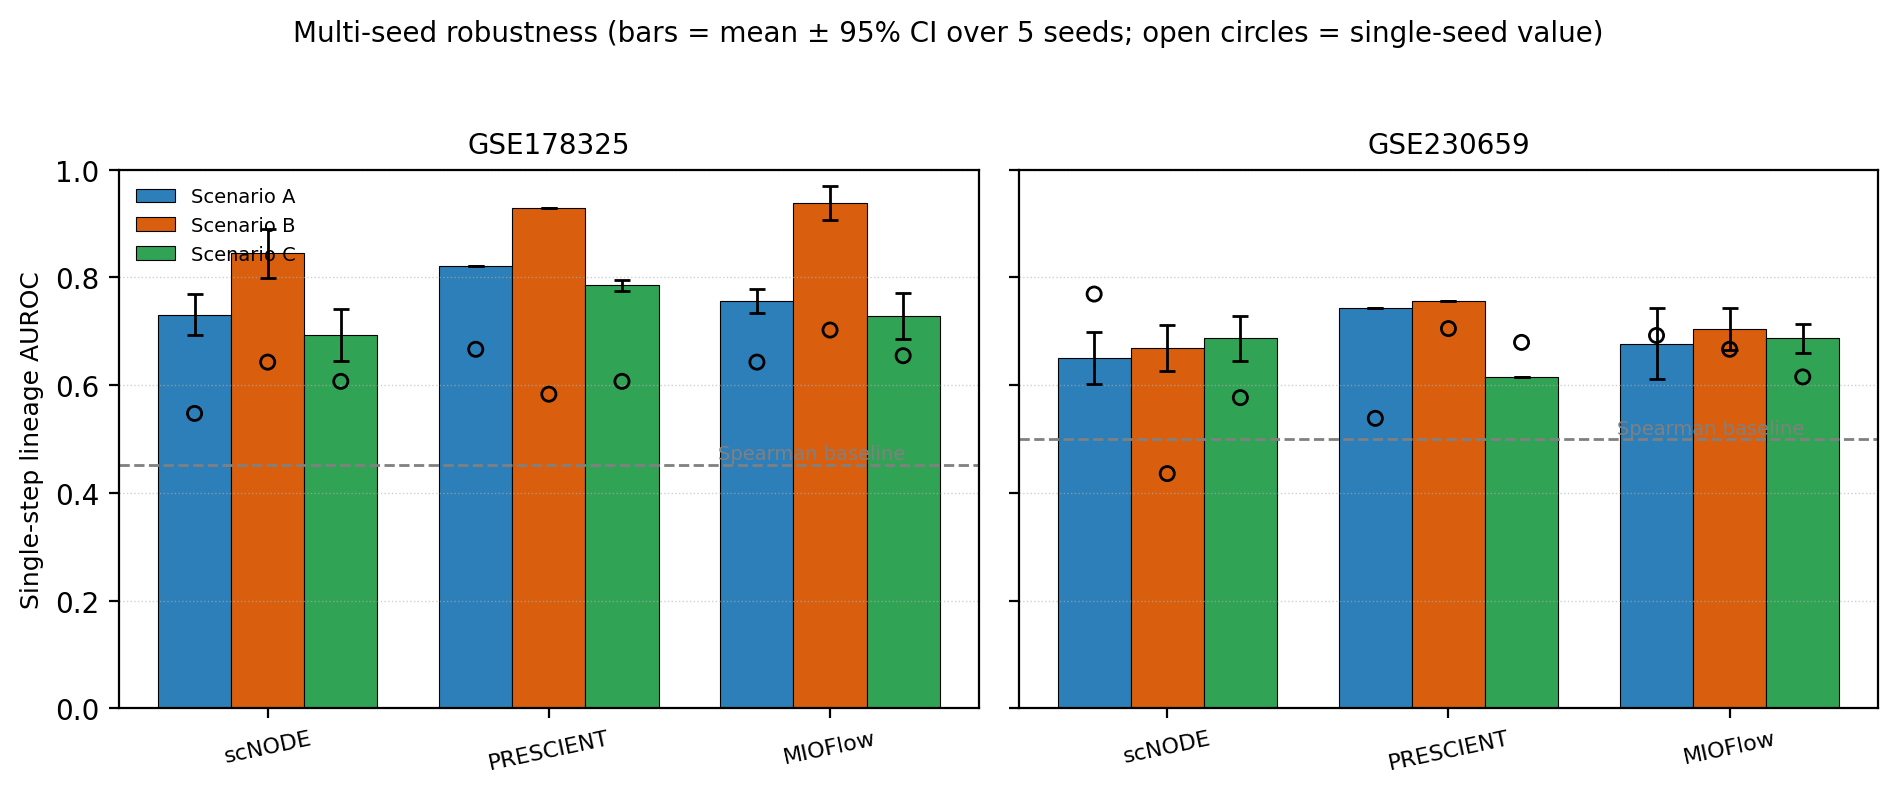
\includegraphics[width=0.95\linewidth]{figures_v2/fig8_multiseed_robustness.png}
\caption{Multi-seed robustness of single-step lineage AUROC on the two primary
datasets. Bars are the mean over five seeds with 95\% confidence intervals; open
circles are the single-seed (seed 42) values reported in the main tables; the dashed
line is the scTimeBench Spearman correlation baseline. Single-seed points often lie
outside the 5-seed interval, and the seed-averaged leader (PRESCIENT) differs from the
single-seed leader (MIOFlow).}
\label{fig:robust}
\end{figure}

\subsection{The scANVI reference gate flags cross-modality transfers that confidence misses}
The reference-construction pipeline (Section~\ref{sec:refval}) is validated against a
positive and a negative control (Fig.~\ref{fig:refval}). The \textbf{positive control}
is a \emph{cross-modality} transfer --- mapping the chemical queries onto the OSKM
reference, which biology says should be rejected: it collapses, with $76$--$96\%$ of query
cells confidently assigned to a single OSKM-transgene state ($<1\%$ of the reference) and
agreement with the existing labels of only $0.01$--$0.04$, yet scANVI's posterior
confidence flags only $\leq0.3\%$ of cells. The geometric OOD gate flags
\textbf{75.9\%/73.0\%} of query cells on the server scANVI latent, correctly catching the
mismatch confidence misses, and the flagged fraction is concentrated in the biologically
plausible states rather than spread uniformly (per-state breakdown in
\code{results/.../ood\_by\_group\_summary.json}). The \textbf{negative controls} show the
gate is not simply pessimistic: a \emph{within-modality} (chemical$\to$chemical) transfer
agrees with the existing annotation at \textbf{0.76--0.86}, and a labeled self-transfer
recovers held-out labels at \textbf{0.944}. The reject decision is stable to the gate's
$k$ and quantile parameters over a sensible range (Section~\ref{sec:refval}). The
benchmark therefore accepts scANVI references only for within-modality transfers that
pass the gate --- exactly the regime in which the cross-modality generalization result
(Fig.~\ref{fig:crosssys}) says references should not be shared. We describe this as a
screened, controlled gate rather than a fully calibrated classifier: the controls bound
its behaviour at the two extremes, but a continuous calibration curve across intermediate
transfer distances is left to future work.

\begin{figure}[ht]
\centering
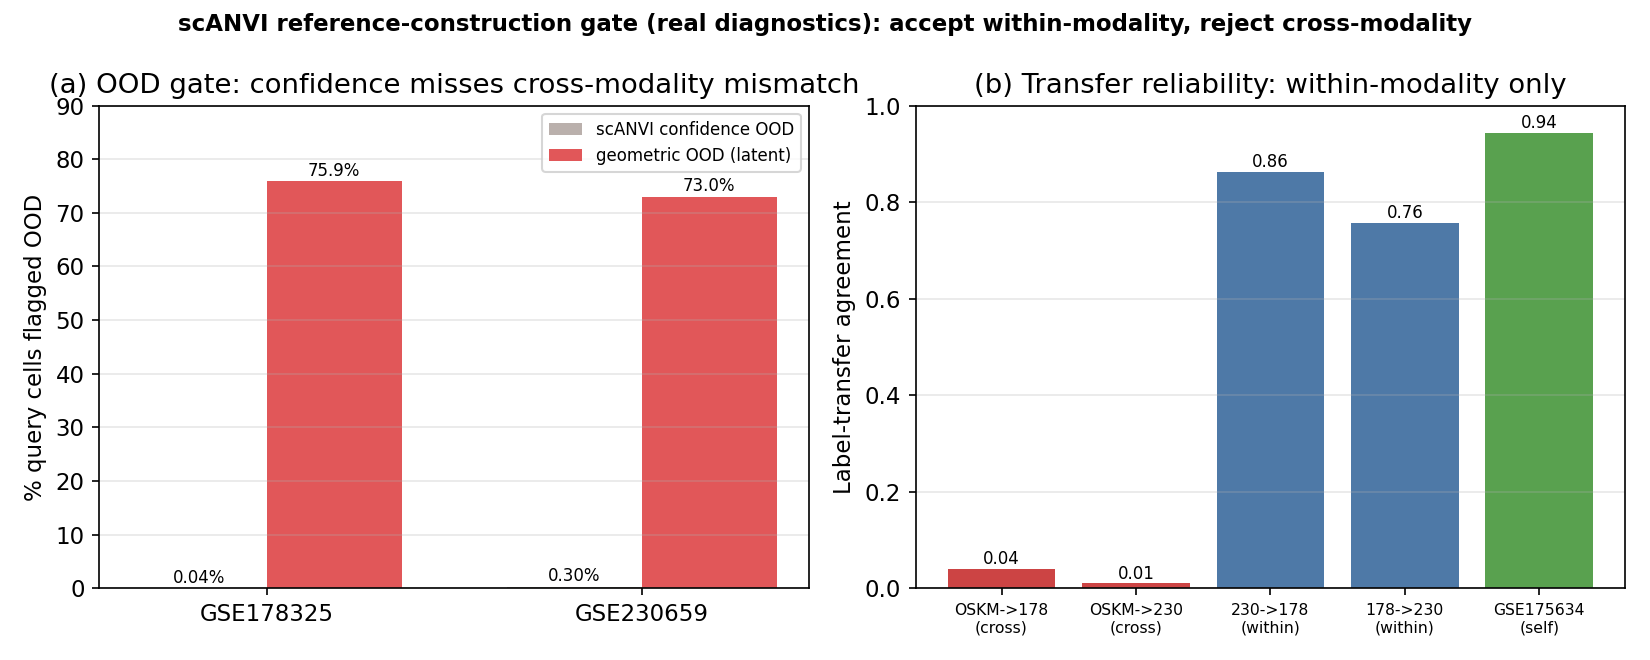
\includegraphics[width=0.95\linewidth]{figures_v2/fig5_scanvi_reference_validation.png}
\caption{scANVI reference-construction gate (real diagnostics). (a) Classifier
confidence flags $\leq0.3\%$ of query cells as out-of-distribution while the geometric
latent OOD score flags $73$--$76\%$ --- confidence is blind to the cross-modality
mismatch. (b) Label-transfer agreement is near zero for cross-modality transfers but
$0.76$--$0.86$ within modality and $0.94$ for a labeled self-transfer; references are
accepted only in the latter regimes.}
\label{fig:refval}
\end{figure}


\subsection{Pseudotime denoises lineage recovery, conditionally}
Replacing the observed-time axis with a diffusion-pseudotime axis (Scenarios
D/E/F) improves lineage fidelity, but the benefit is method- and
system-dependent (Fig.~\ref{fig:ptlineage}). The effect is dramatic for PRESCIENT
on GSE230659, whose mean single-step lineage AUROC rises from $0.64$ on observed
time (A/B/C) to $0.97$ on pseudotime (D/E/F) --- reaching $1.00$ in the joint
Scenario~F --- so that PRESCIENT ranks first in every pseudotime scenario.
MIOFlow gains more modestly on both datasets ($0.66\to0.72$ on GSE230659,
$0.67\to0.76$ on GSE178325), scNODE gains only on GSE178325 ($0.60\to0.69$), and
PRESCIENT is flat on GSE178325 ($0.62\to0.62$). This reproduces scTimeBench's
observation on reprogramming data: pseudotime can denoise the temporal ordering
and sharpen lineage recovery, but the improvement is not guaranteed and is
largest where the observed-time sampling is least informative for a given method.

\begin{figure}[ht]
\centering
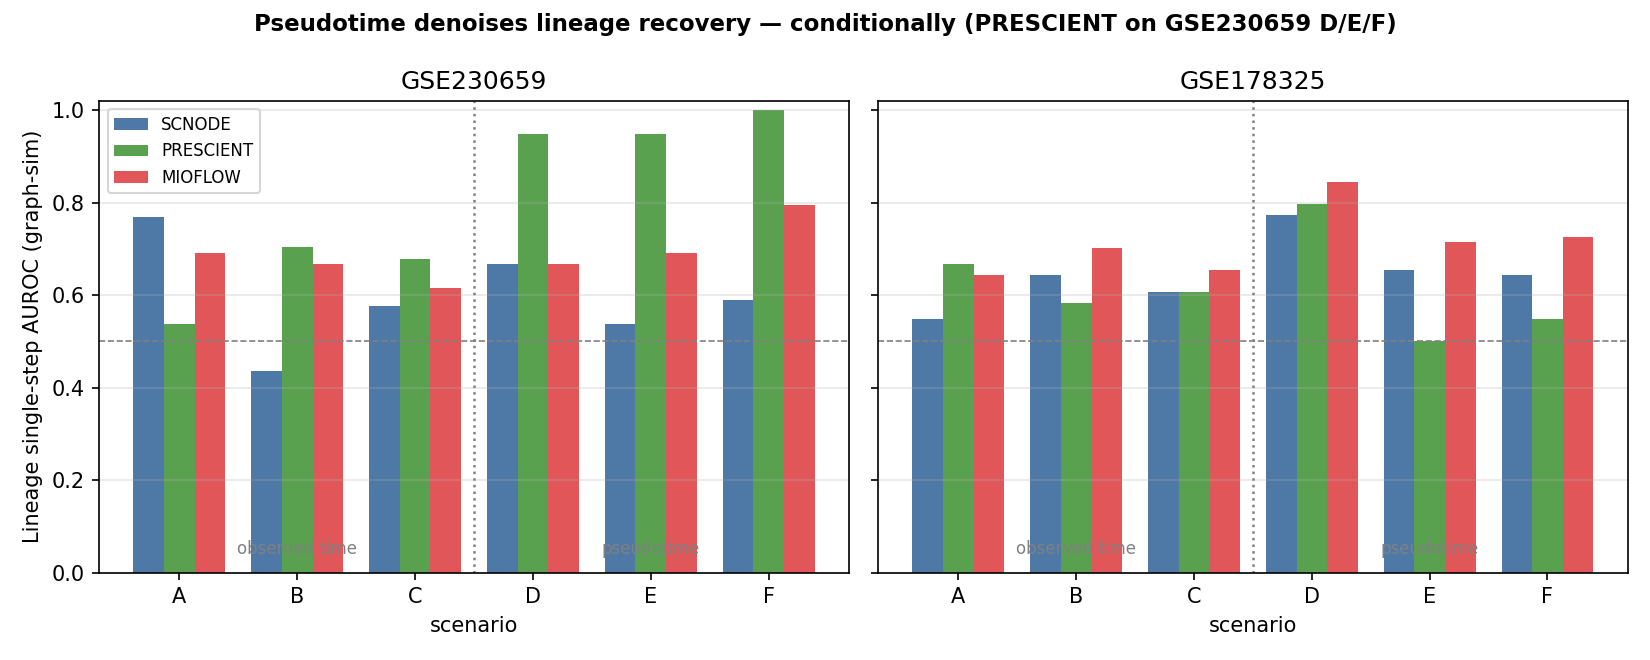
\includegraphics[width=0.95\linewidth]{figures_v2/fig6_pseudotime_lineage.png}
\caption{Pseudotime vs observed time. Single-step lineage AUROC (graph-sim) by
method and scenario; A/B/C use observed time, D/E/F use a 15-bin
diffusion-pseudotime axis (dotted divider). PRESCIENT's lineage recovery on
GSE230659 jumps under pseudotime (to $1.00$ in Scenario~F); gains elsewhere are
milder and method-dependent.}
\label{fig:ptlineage}
\end{figure}

\subsection{Embedding coherence is low in absolute terms}
Absolute embedding ARI is low for all methods ($\leq0.23$; Fig.~\ref{fig:embedding}),
echoing scTimeBench's finding that projected latent spaces often fail to resolve cell
types cleanly. PRESCIENT is most coherent on average, but the ordering changes by
dataset and scenario, so embedding ARI is best read as a relative diagnostic against
the frozen milestone labels.

\begin{figure}[ht]
\centering
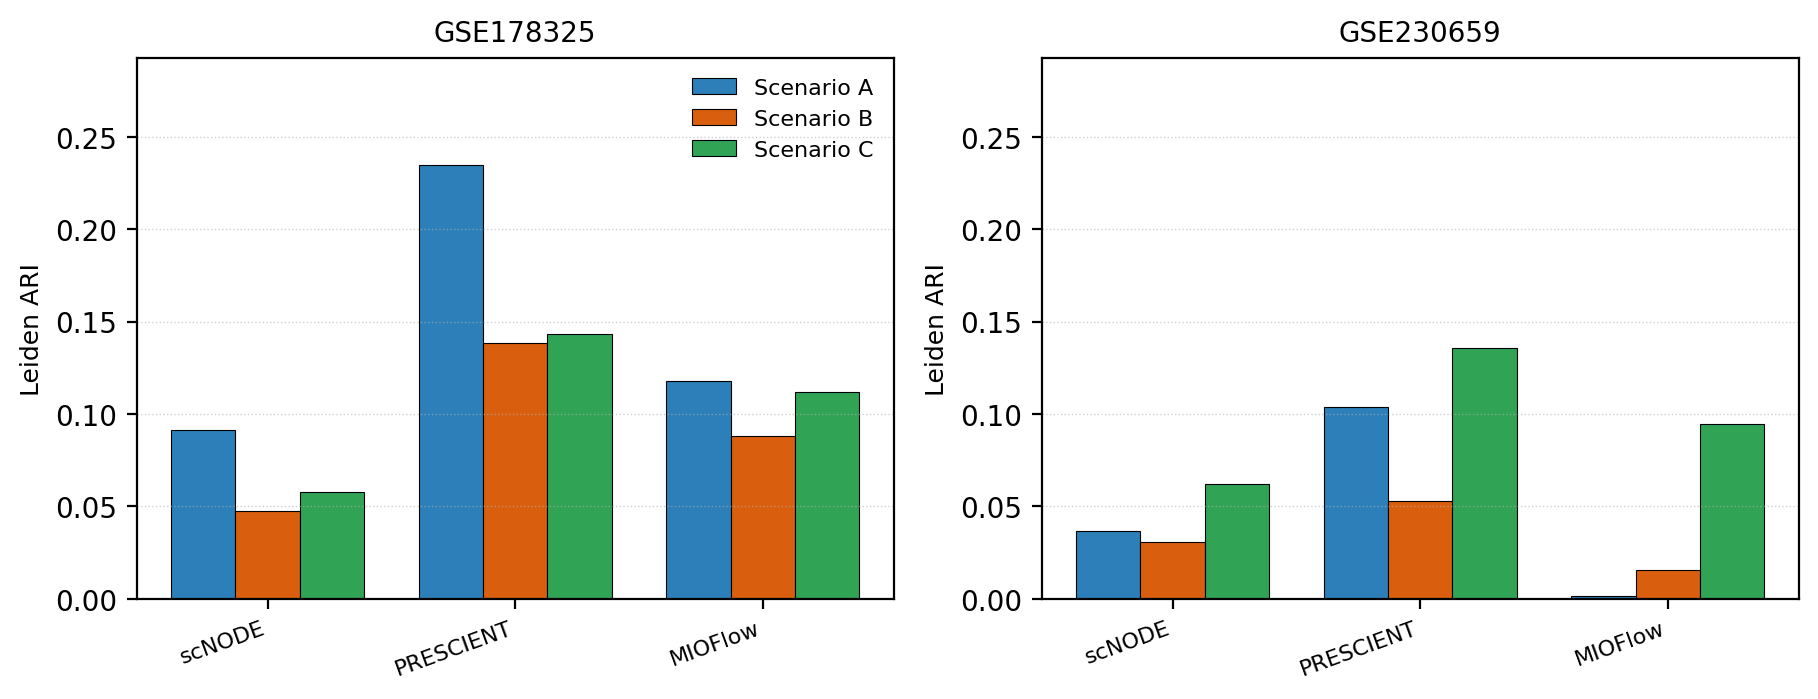
\includegraphics[width=0.95\linewidth]{figures_v2/fig3_embedding_ari.png}
\caption{Embedding Coherence (Leiden-cluster ARI vs reference milestones) by method and
scenario. Absolute ARI is low throughout and the method ordering is not stable across
the two datasets.}
\label{fig:embedding}
\end{figure}

% ------------------------------------------------------------------
\section{Discussion}
% ------------------------------------------------------------------
Narrowing a temporal-trajectory benchmark to the pluripotency domain turns the
question from ``which method wins on average?'' into ``does a method's ranking
transfer across the routes to pluripotency?'', and the answer here is: only for some
tasks. PRESCIENT, MIOFlow, and scNODE trade the lead across forecast, embedding, and
lineage tasks, and all three score substantially higher on OSKM than on chemical
reprogramming. Crucially, the instability is task-dependent: lineage-fidelity rankings
are near-discordant across the four marker-silver systems (Kendall's $W=0.19$),
reversing completely between the human hADSC and mouse systems, whereas forecast
rankings are comparatively portable ($W=0.75$). The non-transfer is therefore not a
blanket caveat but a specific one --- it is the lineage task, the task scTimeBench
already flags as the field's weakest, whose leaderboard is least trustworthy, and it
breaks down along biological axes (species, starting cell type) rather than at random.
Practically, a method should be chosen for the task that matters and validated on a
system close to the target biology --- a lineage-recovery result in particular should
never be read off a single leaderboard. The
reference-construction pipeline makes this domain benchmark feasible despite missing
labels: scANVI/scArches transfer supplies cell-state references, and the geometric OOD
gate --- which catches a confident cross-modality collapse that classifier confidence
entirely misses --- decides when a transferred reference may be used. The two
contributions reinforce each other: the cross-modality generalization result is the
empirical reason the OOD gate refuses cross-modality references.

\paragraph{Scope of the claims.} We frame this work as a \emph{silver-reference benchmark and cautionary analysis}, not a biological-ground-truth study. Every lineage and embedding number is scored against marker-defined or scANVI-transferred references, so the results establish how method rankings behave --- and how fragile they are --- under a transparent, reproducible reference construction, rather than a definitive biological ordering of methods or a mechanism-discovery claim. ``Recovery'' throughout denotes agreement with these frozen coarse reference graphs, not recovery of ground-truth lineage. The three additional generative methods (scIMF, PI-SDE, Squidiff) are planned extensions whose model code is not vendored, raise an explicit \code{VendoringRequired} contract, and contribute to no result in this paper.

\paragraph{Limitations.} Silver references are marker-defined or scANVI-transferred,
not author-validated, so lineage fidelity measures alignment with a coarse reference
graph rather than ground-truth biology; the reference graphs are small (3--4 edges for
the marker-silver systems, 9 for the OSKM author-cluster protocol), so the lineage
metrics are reported with this structural sparsity in mind and the OSKM system, built
under a different reference protocol, is shown stratified rather than pooled with the
marker-silver systems. Four of six datasets carry completed runs across all three tasks
(GSE242424 under the separate author-cluster protocol; GSE175634 carries forecast and
embedding) while the organoid extension needs its own reference; the GSE218855/GSE298212
milestone markers are canonical rather than author-curated and so those two systems are
framed as external stress tests rather than co-equal validation; and PRESCIENT's formal
runs were CPU-only. Multi-seed 95\% confidence intervals are reported for the two primary
datasets (Fig.~\ref{fig:robust}); extending them to the cross-system datasets and the
pseudotime scenarios is the main outstanding analysis, so the headline tables remain
single-seed point estimates that --- as the robustness analysis shows --- should be read
with the seed sensitivity in mind rather than as resolved rankings. The single-seed
combined-rank gaps (e.g.\ $1.79$ vs $1.85$) are therefore descriptive, not statistically
resolved. The three additional generative methods (scIMF, PI-SDE, Squidiff) are scoped as
planned extensions whose model code is not yet vendored, and are excluded from all results.

% ------------------------------------------------------------------
\section{Data and code availability}
\label{sec:repro}
\addcontentsline{toc}{section}{Data and code availability}
All datasets are public (NCBI GEO: GSE178325, GSE230659, GSE242424, GSE175634,
GSE298212, GSE218855; ArrayExpress: E-MTAB-7552). The benchmark framework,
capability-gated evaluators, frozen providers, scANVI/OOD utilities, Shirokane job
scripts, and the scripts that regenerate every table and figure are in the project
repository under \code{benchmark/} and \code{src/}. Each single-seed number reported
here is read directly from a result file under \code{benchmark/reports/},
\code{benchmark/results/}, or \code{results/annotation\_branch/}; the claim-to-source
map is in \code{manuscript/REPRODUCIBILITY.md}. The multi-seed confidence intervals
(Fig.~\ref{fig:robust}) are a \emph{derived} artifact summarised in
\code{multiseed\_ci.csv}. All 90 seed-runs (3 methods $\times$ 2 datasets $\times$
A/B/C $\times$ 5 seeds) executed on the HPC; the run logs
(\code{logs/run\_multiseed\_benchmark.122804086.\{1..90\}.log}) and a SHA-256 checksum
of every seed config (\code{multiseed\_config\_checksums.sha256}) are in the repository,
and \code{multiseed\_manifest.csv} maps each run to its config hash, output directory,
and log. The raw per-seed metric JSONs are not synced (size) but are regenerated by the
documented array recipe in \code{manuscript/REPRODUCIBILITY.md}. Nothing reported here
is fabricated.

% ------------------------------------------------------------------
\begin{thebibliography}{99}
% ------------------------------------------------------------------
\bibitem[Chen et~al.(2023)]{chen2023}
Chen Y, Li S, \emph{et al.}
A fast chemical reprogramming system promotes cell identity transition through a
diapause-like state.
\emph{Nature Cell Biology} 25:1146--1156 (2023).
\href{https://doi.org/10.1038/s41556-023-01193-x}{doi:10.1038/s41556-023-01193-x}.
(GSE218855.)

\bibitem[Elorbany et~al.(2022)]{elorbany2022}
Elorbany R, Popp JM, Rhodes K, \emph{et al.}
Single-cell sequencing reveals lineage-specific dynamic genetic regulation of gene
expression during human cardiomyocyte differentiation.
\emph{PLoS Genetics} 18(1):e1009666 (2022).
\href{https://doi.org/10.1371/journal.pgen.1009666}{doi:10.1371/journal.pgen.1009666}.
(GSE175634.)

\bibitem[Guan et~al.(2022)]{guan2022}
Guan J, Wang G, Wang J, \emph{et al.}
Chemical reprogramming of human somatic cells to pluripotent stem cells.
\emph{Nature} 605:325--331 (2022).
\href{https://doi.org/10.1038/s41586-022-04593-5}{doi:10.1038/s41586-022-04593-5}.
(GSE178325.)

\bibitem[He et~al.(2026)]{he2026squidiff}
He S, Zhu Y, \emph{et al.} Squidiff: predicting cellular development and responses to
perturbations using a diffusion model. \emph{Nature Methods} 23(1):65--77 (2026).
\bibitem[Huguet et~al.(2022)]{huguet2022}
Huguet G, Magruder DS, Tong A, \emph{et al.}
Manifold interpolating optimal-transport flows for trajectory inference (MIOFlow).
\emph{Advances in Neural Information Processing Systems} 35:29705--29718 (2022).
\href{https://doi.org/10.48550/arXiv.2206.14928}{arXiv:2206.14928}.

\bibitem[Jiang et~al.(2026)]{jiang2026scimf}
Jiang Q, Li L, \emph{et al.} Learning collective multicellular dynamics with an
interacting mean field neural SDE model (scIMF). \emph{PLOS Computational Biology}
22(1):e1013916 (2026).
\bibitem[Jiang and Wan(2024)]{jiangwan2024pisde}
Jiang Q, Wan L. A physics-informed neural SDE network for learning cellular dynamics
from time-series scRNA-seq data (PI-SDE). \emph{Bioinformatics} 40(Suppl.~2):ii120--ii127 (2024).
\bibitem[Kanton et~al.(2019)]{kanton2019}
Kanton S, Boyle MJ, He Z, \emph{et al.}
Organoid single-cell genomic atlas uncovers human-specific features of brain
development.
\emph{Nature} 574:418--422 (2019).
\href{https://doi.org/10.1038/s41586-019-1654-9}{doi:10.1038/s41586-019-1654-9}.
(E-MTAB-7552.)

\bibitem[Liuyang et~al.(2023)]{liuyang2023}
Liuyang S, Wang G, Wang Y, \emph{et al.}
Highly efficient and rapid generation of human pluripotent stem cells by chemical
reprogramming.
\emph{Cell Stem Cell} 30:450--459.e9 (2023).
\href{https://doi.org/10.1016/j.stem.2023.02.008}{doi:10.1016/j.stem.2023.02.008}.
(GSE230659.)

\bibitem[Lotfollahi et~al.(2022)]{lotfollahi2022}
Lotfollahi M, Naghipourfar M, Luecken MD, \emph{et al.}
Mapping single-cell data to reference atlases by transfer learning (scArches).
\emph{Nature Biotechnology} 40:121--130 (2022).
\href{https://doi.org/10.1038/s41587-021-01001-7}{doi:10.1038/s41587-021-01001-7}.

\bibitem[Osakwe et~al.(2026)]{osakwe2026}
Osakwe A, Huang EH, Li Y.
scTimeBench: a streamlined benchmarking platform for single-cell time-series analysis.
\emph{bioRxiv} (2026).
\href{https://doi.org/10.64898/2026.03.16.712069}{doi:10.64898/2026.03.16.712069}.

\bibitem[Peng et~al.(2025)]{peng2025}
Peng F, \emph{et al.}
Chemical reprogramming of human blood cells to pluripotent stem cells.
\emph{Cell Stem Cell} 32:1192--1199.e11 (2025).
\href{https://doi.org/10.1016/j.stem.2025.07.003}{doi:10.1016/j.stem.2025.07.003}.
(GSE298212.)

\bibitem[Schiebinger et~al.(2019)]{schiebinger2019}
Schiebinger G, Shu J, Tabaka M, \emph{et al.}
Optimal-transport analysis of single-cell gene expression identifies developmental
trajectories in reprogramming (Waddington-OT).
\emph{Cell} 176:928--943.e22 (2019).
\href{https://doi.org/10.1016/j.cell.2019.01.006}{doi:10.1016/j.cell.2019.01.006}.
(GSE115943.)

\bibitem[Weiler et~al.(2024)]{weiler2024}
Weiler P, Lange M, Klein M, Pe'er D, Theis FJ.
CellRank 2: unified fate mapping in multiview single-cell data.
\emph{Nature Methods} 21:1196--1205 (2024).
\href{https://doi.org/10.1038/s41592-024-02303-9}{doi:10.1038/s41592-024-02303-9}.

\bibitem[Xu et~al.(2021)]{xu2021}
Xu C, Lopez R, Mehlman E, Regier J, Jordan MI, Yosef N.
Probabilistic harmonization and annotation of single-cell transcriptomics data with
deep generative models (scANVI).
\emph{Molecular Systems Biology} 17:e9620 (2021).
\href{https://doi.org/10.15252/msb.20209620}{doi:10.15252/msb.20209620}.

\bibitem[Yeo et~al.(2021)]{yeo2021}
Yeo GHT, Saksena SD, Gifford DK.
Generative modeling of single-cell time series with PRESCIENT.
\emph{Nature Communications} 12:3222 (2021).
\href{https://doi.org/10.1038/s41467-021-23518-w}{doi:10.1038/s41467-021-23518-w}.

\bibitem[Zhang et~al.(2024)]{zhang2024scnode}
Zhang J, Larschan E, Bigness J, Singh R.
scNODE: generative model for temporal single-cell transcriptomic data prediction.
\emph{Bioinformatics} 40(Suppl.~2):ii146--ii154 (2024).
\href{https://doi.org/10.1093/bioinformatics/btae393}{doi:10.1093/bioinformatics/btae393}.

\end{thebibliography}

\end{document}
